\documentclass{WCCM-ECCOMAS_2026_Full_Paper}

\usepackage{graphicx}
\usepackage{amsmath}
\usepackage{amssymb}
\usepackage{booktabs}
\usepackage{xcolor}
\usepackage[colorlinks=true,linkcolor=blue,urlcolor=blue,citecolor=blue]{hyperref}

% ---------------------------------------------------------------
% Placeholder commands for values to be filled from experiments
% ---------------------------------------------------------------
\newcommand{\result}[1]{\textcolor{red}{\textbf{[#1]}}}
\newcommand{\figplaceholder}[1]{%
  \fbox{\parbox{0.95\linewidth}{\centering\vspace{1.5cm}%
  \textit{\small [Figure placeholder: #1]}\vspace{1.5cm}}}%
}

% ---------------------------------------------------------------
% Title — all caps per ECCOMAS format
% ---------------------------------------------------------------
\title{Physics-Aware Mixture of Experts for High-Fidelity Shock Capture in Transonic Aerodynamic Surface Prediction}

\author{Marta Arnabat-Martín$^{*}$, Andrés Mateo-Gabín$^{\P}$, Sven A. Lanzan-Ferran$^{\P}$ and Gonzalo Rubio$^{\dag}$}
\shortauthors{Marta Arnabat-Martín}

\address{%
$^{*}$ Flight Physics Technology and Capability\\
Airbus Defence and Space, C/ Aviocar 2, 28906 Getafe, Madrid, Spain \\
Universidad Politécnica de Madrid, Plaza Cardenal Cisneros, 3, Madrid, 28040, Spain\\
e-mail: marta.arnabt-martin@airbus.com \\[12pt]

$^{\P}$ Flight Physics Technology and Capability\\
Airbus Defence and Space, C/ Aviocar 2, 28906 Getafe, Madrid, Spain \\
e-mail: andres.mateo@airbus.com \\
e-mail: sven\_agustin-lanzan@airbus.com \\[12pt]
$^{\dag}$ Applied Mathematics department - School of aeronautics\\
Universidad Politécnica de Madrid, Plaza Cardenal Cisneros, 3, Madrid, 28040, Spain\\
Center of Computational Simulation, Universidad Politécnica de Madrid, Campus de Montegancedo, Boadilla del Monte, 28660 Madrid, Spain

}

\keywords{shock detection, mixture of experts, sparse autoencoder,
symbolic regression, physics-informed machine learning, RANS surrogate}

\summary{A physics-informed machine learning pipeline
is presented for interpretable shock and flow-separation detection on
aerodynamic surface data, requiring no CFD solver at inference.
A Sparse Autoencoder~(SAE) encodes surface flow state into a compact
latent representation; a Mixture of Experts~(MoE) exploits this
representation for regime-aware aerodynamic coefficient prediction; and
a Virtual Shock Sensor~(VSS) infers shock probability and separation
probability from the latent state and flight-condition inputs alone.
All training labels are derived from real RANS surface quantities---no
isentropic pseudo-labels are used.  Post-training Symbolic Regression
recovers a closed-form shock equation from eight physical input
features, providing human-readable interpretability.  Trained on 81
million surface points from 468 RANS simulations of the ONERA CRM
WBPN configuration spanning Mach $0.3$--$0.9$ and angle of attack
$\pm 15^{\circ}$, the pipeline achieves AUC-ROC of \result{X.XX} for
shock detection, while the recovered symbolic equation is dominated by
Mach number and the critical pressure coefficient, confirming that
genuine shock physics have been learned.}

\begin{document}
\maketitle

% ================================================================
\section{INTRODUCTION}
% ================================================================

Transonic aerodynamic flows are characterised by the coexistence of
subsonic and supersonic regions separated by shock waves.  In cruise
configurations, normal shocks on wing surfaces produce strong adverse
pressure gradients that drive boundary-layer thickening, flow
separation, and buffet onset---phenomena central to the determination
of drag-divergence Mach number and the structural loads
envelope~\cite{Vassberg2008,Levy2013}.  Accurate, low-cost detection
of shock location and intensity is therefore a fundamental requirement
for aerodynamic analysis pipelines that must operate at high
frequency, such as adjoint-based shape optimisation, digital-twin
monitoring, or real-time loads estimation.

Reynolds-Averaged Navier--Stokes (RANS) solvers provide physical
ground truth for shock structure but at a computational cost of
$\mathcal{O}(10^{3}$--$10^{4})$ CPU-hours per operating condition.
Machine learning (ML) surrogate models have emerged as a practical
alternative for rapid aerodynamic
prediction~\cite{Han2018,Bhatnagar2019,Sekar2019}.  A central
challenge in transonic aerodynamics is regime non-uniformity: the
relationship between surface geometry, flight condition, and
aerodynamic loading changes qualitatively across subsonic, transonic,
and separated flow regimes.  A single multi-layer perceptron (MLP)
trained on data spanning all regimes learns a smooth interpolant that
systematically blurs shock discontinuities, underestimating peak
suction and misrepresenting the pressure-recovery gradient aft of the
shock.

Existing ML shock indicators address this at the volumetric field
level.  Ray and Hesthaven~\cite{Ray2018,Ray2019} pioneered neural
network troubled-cell indicators for finite-element solution fields;
Discacciati et al.~\cite{Discacciati2020} and Schwander et
al.~\cite{Schwander2021} extended these with convolutional
architectures.  Morgan et al.~\cite{Morgan2020} developed
field-level indicators for Lagrangian hydrodynamics.  Two limitations
are shared across these approaches: (i)~they require volumetric field
data inaccessible in the surface-only measurement context of
experimental aerodynamics or flight test, and (ii)~they commonly rely
on pseudo-labels derived from isentropic assumptions applied to input
features, introducing a definitional circularity.  Physics-informed
neural networks~\cite{Raissi2019,Karniadakis2021} offer an
alternative route but require embedding governing equations explicitly
and are computationally intensive to train.

The interpretability of ML models for physical discovery constitutes
a parallel active frontier.  Symbolic regression (SR)
methods---SINDy~\cite{Brunton2016}, Eureqa~\cite{Schmidt2009}, and
PySR~\cite{Cranmer2020}---have demonstrated that compact,
human-readable governing equations can be recovered from data, and
recent benchmarks~\cite{LaCava2021,Angelis2023} have shown their
maturity across physical domains.  However, their application to
aerodynamic shock physics at industrial scale has not been
demonstrated.

This work addresses both gaps simultaneously.  We present a
four-component pipeline: (i)~a Sparse Autoencoder~(SAE) that encodes
surface flow state into a compact, disentangled latent representation;
(ii)~a Mixture of Experts~(MoE) that predicts aerodynamic coefficients
in a regime-aware manner; (iii)~a Virtual Shock Sensor~(VSS) trained
on labels derived entirely from real RANS solver output, producing
shock and separation probabilities from surface geometry and flight
condition alone; and (iv)~a post-training symbolic regression stage
that distils learned knowledge into a closed-form equation operable
without any ML tooling.

The four main contributions of this work are:
\begin{enumerate}
  \item A sparse autoencoder trained on 81 million RANS surface points
        that learns a low-dimensional, disentangled representation of
        aerodynamic surface state across 468 flight conditions
        (Mach~$0.3$--$0.9$, AoA~$\pm 15^{\circ}$).
  \item A Mixture of Experts architecture whose gate weights emerge as
        empirically interpretable aerodynamic regime classifiers,
        avoiding the shock-smoothing pathology of single-MLP
        surrogates.
  \item A Virtual Shock Sensor trained exclusively on CFD-derived
        labels that infers shock and separation probability from
        surface geometry and flight-condition inputs, requiring no
        solver at inference.
  \item Recovery of a closed-form shock equation via symbolic
        regression, providing physical interpretability and enabling
        lightweight deployment.
\end{enumerate}

% ================================================================
\section{DATASET AND PROBLEM FORMULATION}
% ================================================================

\subsection{Configuration and simulation database}

The ONERA Common Research Model Wing--Body--Pylon--Nacelle
(CRM~WBPN)~\cite{Vassberg2008,Levy2013} is a high-fidelity
industry-standard benchmark for transonic transport aerodynamics.
A database of 468 steady RANS simulations is assembled, spanning
freestream Mach number $M \in [0.30,\,0.90]$ and angle of attack
$\alpha \in [-15^{\circ},\,+15^{\circ}]$, with total pressure $\Pi$
sampled to represent a representative altitude envelope.  All
simulations employ the $k$--$\omega$~SST turbulence model on a
structured surface mesh.  Surface data---pressure coefficient $C_p$
and skin-friction components $C_{fx}$, $C_{fy}$, $C_{fz}$---are
extracted at all mesh nodes, yielding approximately 121 million
surface points.  The dataset is partitioned \emph{at the simulation
level} into 374 training simulations (81\,M~points) and 94 test
simulations (40\,M~points), ensuring no flight condition seen at
training time appears in the test set.  Key statistics are summarised
in Table~\ref{tab:dataset}.

\begin{table}[ht]
\centering
\caption{Simulation database statistics for the ONERA CRM WBPN.}
\label{tab:dataset}
\begin{tabular}{lcc}
\toprule
\textbf{Quantity} & \textbf{Training set} & \textbf{Test set} \\
\midrule
Simulations        & 374                  & 94                \\
Surface points     & 81\,000\,000         & 40\,000\,000      \\
Mach range         & $[0.30,\;0.90]$      & $[0.30,\;0.90]$   \\
AoA range          & $[-15^{\circ},\;+15^{\circ}]$ & $[-15^{\circ},\;+15^{\circ}]$ \\
Shocked points (\%)   & \result{XX.X}     & \result{XX.X}     \\
Separated points (\%) & \result{XX.X}     & \result{XX.X}     \\
\bottomrule
\end{tabular}
\end{table}

\subsection{Feature engineering}

Each surface point is characterised by nine base features:
\begin{equation}
  \mathbf{x}_{\mathrm{base}}
  = \bigl[x,\;y,\;z,\;n_x,\;n_y,\;n_z,\;M,\;\alpha,\;
          \Pi{\times}10^{-5}\bigr]
  \in \mathbb{R}^{9}
  \label{eq:xbase}
\end{equation}
where $(x,y,z)$ are surface coordinates normalised by the reference
chord, $(n_x,n_y,n_z)$ is the outward unit normal, $M$ is the
freestream Mach number, $\alpha$ is the angle of attack in degrees,
and $\Pi$ is the freestream total pressure.  Five physics-derived
features are appended, each computed from $\mathbf{x}_{\mathrm{base}}$
alone:
\begin{equation}
  q_{\mathrm{dyn}} = \frac{\gamma\,\Pi\,M^{2}}
    {2\!\left(1+\tfrac{\gamma-1}{2}M^{2}\right)^{\!\gamma/(\gamma-1)}},
  \qquad
  \Pi_{\mathrm{norm}} = \frac{\Pi}{\Pi_{\mathrm{ref}}},
  \qquad
  \mathrm{AoA}_{\sin} = \sin\alpha
  \label{eq:derived1}
\end{equation}
\begin{equation}
  L_{\mathrm{factor}} = M^{2}\sin\alpha,
  \qquad
  C_{p}^{\mathrm{crit}}(M) =
    \frac{2}{\gamma M^{2}}\!\left[
      \left(\frac{2}{\gamma+1}+\frac{\gamma-1}{\gamma+1}M^{2}\right)^{\!\!
        \gamma/(\gamma-1)}\!\!\!-\,1\right]
  \label{eq:cpcrit}
\end{equation}
where $\gamma = 1.4$ for air and $\Pi_{\mathrm{ref}}$ is a reference
total pressure.  The quantity $C_{p}^{\mathrm{crit}}$ is the pressure
coefficient at the sonic condition ($M_{\mathrm{local}}=1$) derived
from isentropic relations.  The full input vector
$\mathbf{x}\in\mathbb{R}^{14}$ concatenates both groups; all derived
features require only $\mathbf{x}_{\mathrm{base}}$---no solver output
enters at the feature-engineering stage.  Table~\ref{tab:features}
lists all fourteen features with their physical interpretation.

\begin{table}[ht]
\centering
\caption{Complete feature set $\mathbf{x}\in\mathbb{R}^{14}$.
  The lower block is computed from the upper block only; no RANS
  output is used.}
\label{tab:features}
\begin{tabular}{lll}
\toprule
\textbf{Feature} & \textbf{Group} & \textbf{Physical meaning} \\
\midrule
$x,\;y,\;z$        & Base & Normalised surface coordinates \\
$n_x,\;n_y,\;n_z$ & Base & Outward unit normal components \\
$M$                & Base & Freestream Mach number \\
$\alpha$           & Base & Angle of attack (deg) \\
$\Pi{\times}10^{-5}$ & Base & Freestream total pressure \\
\midrule
$q_{\mathrm{dyn}}$    & Derived & Isentropic dynamic pressure (Eq.~\ref{eq:derived1}) \\
$\Pi_{\mathrm{norm}}$ & Derived & Normalised total pressure \\
$\mathrm{AoA}_{\sin}$ & Derived & $\sin(\alpha)$, lift-relevant projection \\
$L_{\mathrm{factor}}$ & Derived & $M^{2}\sin\alpha$, coupled lift--Mach parameter \\
$C_{p}^{\mathrm{crit}}$ & Derived & Critical Cp at sonic condition (Eq.~\ref{eq:cpcrit}) \\
\bottomrule
\end{tabular}
\end{table}

\subsection{Label generation from RANS output}

Two binary labels are defined for each surface point using RANS solver
outputs \[ \mathbf{y} = [C_{p},C_{fx},C_{fy},C_{fz}] \]
\begin{equation}
  y_{\mathrm{shock}} =
    \mathbf{1}\!\left[C_{p}^{\mathrm{RANS}} < C_{p}^{\mathrm{crit}}(M)\right],
  \qquad
  y_{\mathrm{sep}} =
    \mathbf{1}\!\left[C_{fx} < 0\right]
  \label{eq:labels}
\end{equation}
The shock label identifies surface points where the RANS-predicted
pressure coefficient falls below the sonic threshold---the condition
for a locally supersonic boundary layer.  Critically,
$C_{p}^{\mathrm{RANS}}$ is a solver output embedding viscous,
turbulent, and compressibility effects; the threshold
$C_{p}^{\mathrm{crit}}$ is a well-established physical criterion, not
a model assumption applied to the inputs.  This distinguishes our
labelling strategy from pseudo-label approaches that derive shock
indicators directly from~$\mathbf{x}_{\mathrm{base}}$.  The
separation label identifies regions of reversed streamwise skin
friction.

% ================================================================
\section{METHODOLOGY}
% ================================================================

The pipeline consists of three trainable components arranged
sequentially---SAE, MoE, and VSS---plus a post-training symbolic
regression stage.  Figure~\ref{fig:architecture} illustrates the
complete data flow and the boundary between the training-time and
inference-time paths.

\begin{figure}[ht]
\centering
%\figplaceholder{Full pipeline: X $\to$ SAE encoder $\to$ latent
%  $\mathbf{z}$ $\to$ MoE (Cp/Cf prediction) and VSS (shock/sep
%  inference) $\to$ SR (closed-form equation).  Annotate the
%  inference boundary: only $\mathbf{x}$ is required at deployment.}
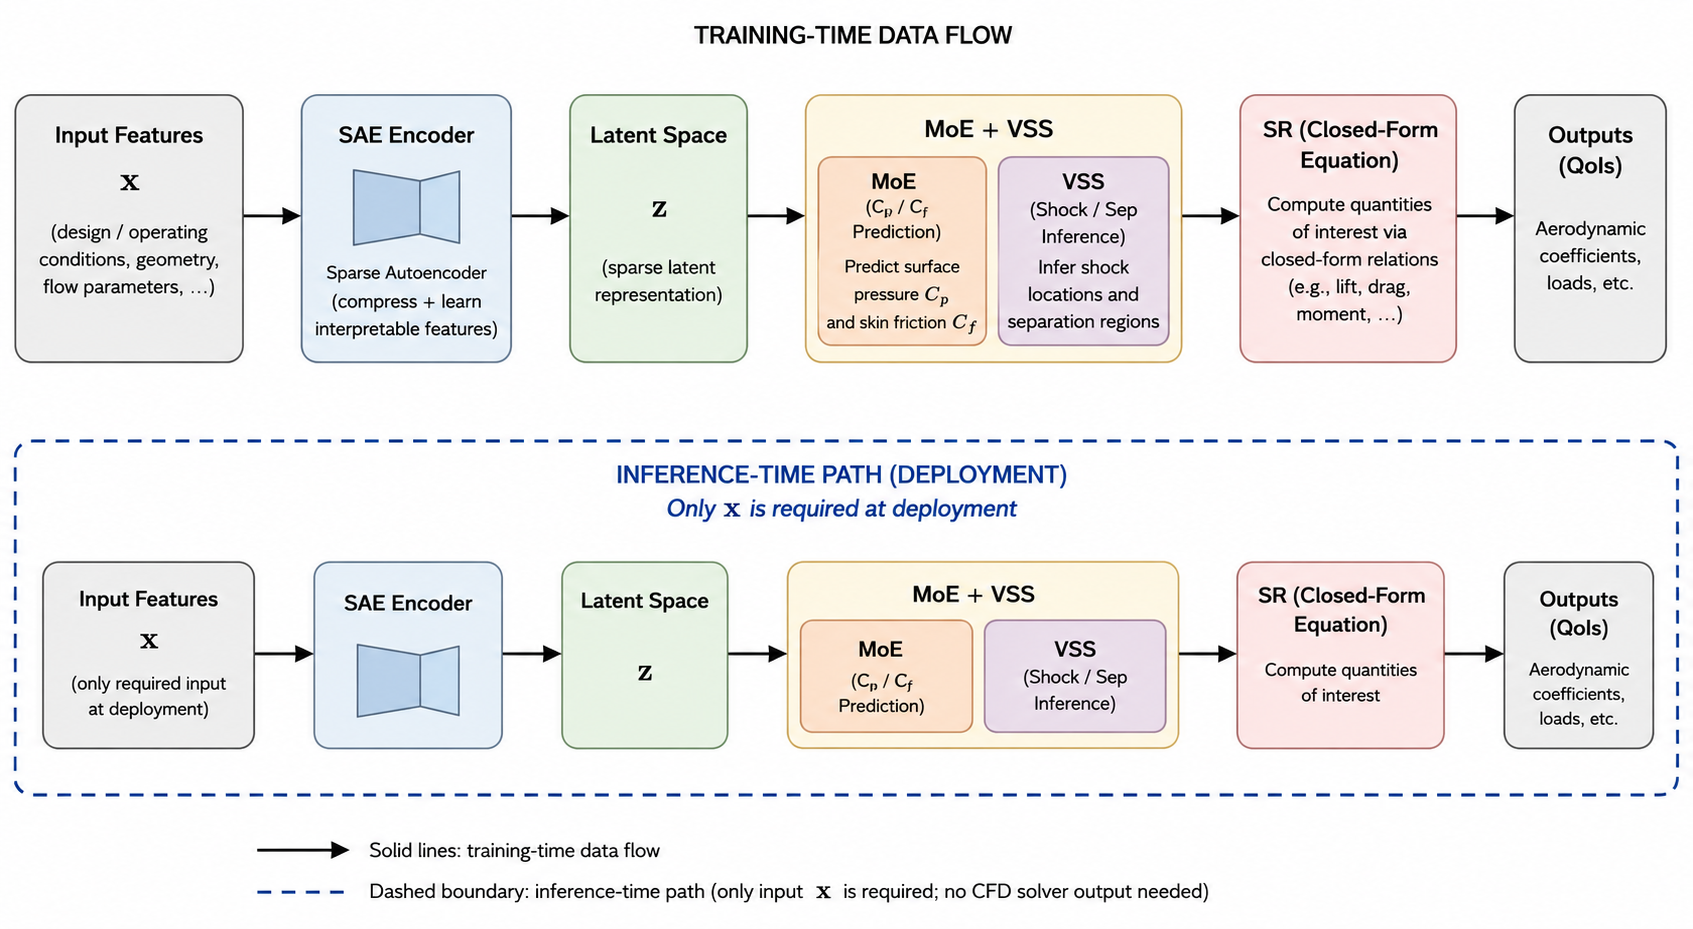
\includegraphics[width=1.0\textwidth]{figures/Pipeline.png}
\caption{Complete SAE--MoE--VSS pipeline.  Solid lines indicate the
  training-time data flow; the dashed boundary marks the
  inference-time path, which requires only the input feature vector
  $\mathbf{x}$ and no CFD solver output.}
\label{fig:architecture}
\end{figure}

\subsection{Sparse Autoencoder (SAE)}
\label{sec:sae}

The SAE maps each input $\mathbf{x}\in\mathbb{R}^{14}$ to a latent
code $\mathbf{z}\in\mathbb{R}^{32}$ and back to a reconstruction
$\hat{\mathbf{x}}$~\cite{Vincent2010,Goodfellow2016}:
\begin{equation}
  \mathbf{z} = \mathrm{Enc}(\mathbf{x};\,\theta_{e}),
  \qquad
  \hat{\mathbf{x}} = \mathrm{Dec}(\mathbf{z};\,\theta_{d})
\end{equation}
The encoder is a three-layer MLP with architecture
$14\!\to\!128\!\to\!64\!\to\!32$ (ReLU activations); the decoder
mirrors this structure.  Training minimises:
\begin{equation}
  \mathcal{L}_{\mathrm{SAE}} =
    \|\mathbf{x} - \hat{\mathbf{x}}\|_{2}^{2}
    + \lambda\,\|\mathbf{z}\|_{1}
  \label{eq:saeloss}
\end{equation}
The $\ell_{1}$ penalty promotes sparsity in the latent code:
most dimensions remain inactive for a given input, and each active
dimension captures a distinct aspect of local flow state.  This
disentanglement serves two downstream purposes: it improves the
physical interpretability of the MoE gating network, and it
simplifies the feature space on which symbolic regression must operate.

\subsection{Mixture of Experts (MoE)}
\label{sec:moe}

The MoE takes the latent code $\mathbf{z}$ and predicts surface
aerodynamic coefficients
$\hat{\mathbf{y}}=[\hat{C}_{p},\hat{C}_{fx},\hat{C}_{fy},\hat{C}_{fz}]$.
It comprises $K=4$ expert networks $\{f_{k}\}_{k=1}^{4}$ and a soft
gating network~$g$~\cite{Jacobs1991,Shazeer2017}:
\begin{equation}
  \hat{\mathbf{y}} =
    \sum_{k=1}^{K} g_{k}(\mathbf{z})\,f_{k}(\mathbf{z};\,\phi_{k}),
  \qquad
  \mathbf{g}(\mathbf{z}) = \mathrm{softmax}(W_{g}\mathbf{z}+\mathbf{b}_{g})
  \label{eq:moe}
\end{equation}
Each expert is a two-layer MLP ($32\!\to\!256\!\to\!32$, ReLU) followed
by a linear output head.  Training minimises:
\begin{equation}
  \mathcal{L}_{\mathrm{MoE}} =
    \|\mathbf{y}-\hat{\mathbf{y}}\|_{2}^{2}
    + \mu\sum_{k=1}^{K}\bar{g}_{k}\log\bar{g}_{k}
  \label{eq:moeloss}
\end{equation}
where $\bar{g}_{k}$ is the batch-averaged gate weight for expert~$k$
and the second term is an auxiliary load-balancing penalty that
prevents gate collapse.  The gate weights $g_{k}(\mathbf{z})$ are the
key interpretability lever: if each expert spontaneously specialises on
a physically distinct flow regime, the gate constitutes an
\emph{emergent} regime classifier---a property verified in
Section~\ref{sec:gateanalysis}.

\subsection{Virtual Shock Sensor (VSS)}
\label{sec:vss}

The VSS is a multi-task network conditioned on the concatenated vector
$[\mathbf{z};\,M;\,\alpha]\in\mathbb{R}^{34}$ and produces three
outputs through separate prediction heads:
\begin{equation}
  \bigl[\hat{p}_{\mathrm{shock}},\;\hat{s}_{\mathrm{int}},\;
        \hat{p}_{\mathrm{sep}}\bigr]
  = \mathrm{VSS}\!\bigl([\mathbf{z};\,M;\,\alpha];\,\psi\bigr)
  \label{eq:vss}
\end{equation}
where $\hat{p}_{\mathrm{shock}}\in[0,1]$ is the shock probability
(sigmoid head, binary cross-entropy loss on $y_{\mathrm{shock}}$),
$\hat{s}_{\mathrm{int}}\geq 0$ is the shock intensity (linear head,
MSE loss), and $\hat{p}_{\mathrm{sep}}\in[0,1]$ is the separation
probability (sigmoid head, binary cross-entropy loss on
$y_{\mathrm{sep}}$).  The two class-probability heads share a common
trunk ($34\!\to\!128\!\to\!64$, ReLU).

At inference, $\mathbf{z}=\mathrm{Enc}(\mathbf{x};\,\theta_{e})$ is
obtained from the frozen SAE encoder, and $M$, $\alpha$ are
components of $\mathbf{x}_{\mathrm{base}}$.  The complete inference
path therefore reads $\mathbf{x}\to\mathbf{z}\to\hat{p}_{\mathrm{shock}}$
and requires no RANS output.  Table~\ref{tab:arch} collects all
architectural and training hyperparameters.

\begin{table}[ht]
\centering
\caption{Architecture and training hyperparameters.}
\label{tab:arch}
\begin{tabular}{lll}
\toprule
\textbf{Component} & \textbf{Parameter} & \textbf{Value} \\
\midrule
SAE   & Encoder / Decoder layers  & $14{\to}128{\to}64{\to}32$ / mirror \\
      & Sparsity weight~$\lambda$ & \result{X.XX} \\
      & Activation                & ReLU \\
\midrule
MoE   & Experts $K$               & 4 \\
      & Expert layers             & $32{\to}256{\to}32$ \\
      & Load-balance weight $\mu$ & \result{X.XX} \\
\midrule
VSS   & Input / trunk layers      & $34{\to}128{\to}64$ \\
      & Output heads              & 3 (shock prob., intensity, sep.\ prob.) \\
\midrule
All   & Optimiser                 & Adam ($\beta_1=0.9$, $\beta_2=0.999$) \\
      & Learning rate             & \result{X.XXe-X} \\
      & Batch size                & \result{XXXX} \\
      & Epochs (SAE / MoE / VSS)  & \result{X / X / X} \\
\bottomrule
\end{tabular}
\end{table}

% ================================================================
\section{SYMBOLIC REGRESSION FOR PHYSICAL INTERPRETABILITY}
\label{sec:sr}
% ================================================================

Post-training, symbolic regression is applied to recover a closed-form
algebraic expression that predicts $y_{\mathrm{shock}}$ from a subset
of eight physically meaningful features:
\[\mathbf{x}_{\mathrm{sr}} = [M,\,\alpha,\,q_{\mathrm{dyn}},\,
\Pi_{\mathrm{norm}},\,\mathrm{AoA}_{\sin},\,L_{\mathrm{factor}},\,
C_{p}^{\mathrm{crit}},\,n_{z}]\] Geometric coordinates $(x,y,z)$ and
raw normal components $(n_x,n_y)$ are excluded to promote discovery
of a condition based on flow physics rather than surface location.

\subsection{PySR setup}

PySR~\cite{Cranmer2020} performs multi-objective evolutionary search
over expression trees, minimising:
\begin{equation}
  \mathcal{L}_{\mathrm{SR}}(f) =
    \mathrm{MSE}\!\bigl(f(\mathbf{x}_{\mathrm{sr}}),\,
                        \hat{p}_{\mathrm{shock}}\bigr)
    + \beta\cdot\mathrm{Complexity}(f)
  \label{eq:sr}
\end{equation}
where the target is the VSS-predicted shock probability
$\hat{p}_{\mathrm{shock}}$ (a noise-regularised surrogate for
$y_{\mathrm{shock}}$), $\mathrm{Complexity}$ counts expression-tree
nodes, and $\beta$ is a complexity penalty.  Allowed operators are
$\{+,\,-,\,\times,\,\div,\,\exp,\,\log,\,|\cdot|\}$.  A Decision Tree
with depth~3 is also trained in parallel on the same feature set as a
fast interpretable baseline.

\subsection{Expression selection and validation}

The result is a Pareto front of expressions trading accuracy against
complexity.  The expression at the inflection point of the front is
selected---the smallest model at which accuracy saturates.

We anticipate---and will confirm empirically---that the dominant terms
involve $M$ and $C_{p}^{\mathrm{crit}}(M)$, consistent with the
isentropic shock criterion.  The general expected form is:
\begin{equation}
  \hat{y}_{\mathrm{shock}}^{\mathrm{SR}} =
    \sigma\!\left(w_{1} C_{p}^{\mathrm{crit}}(M)
                 + w_{2} q_{\mathrm{dyn}}
                 + w_{3} M^{2} + b\right)
  \label{eq:srform}
\end{equation}
If SR independently recovers a combination dominated by
$C_{p}^{\mathrm{crit}}$ and $M$, this constitutes a data-driven
falsification test: the network has learned genuine shock physics,
not a spurious geometric correlation.  The recovered expression is
evaluated on the 40\,M-point test set and compared against the full
VSS network and the isentropic baseline
$\mathbf{1}[C_{p}^{\mathrm{crit}}(M) < 0]$.

% ================================================================
\section{RESULTS AND DISCUSSION}
\label{sec:results}
% ================================================================

\subsection{Coefficient prediction accuracy}

Table~\ref{tab:results} reports prediction accuracy for all four
surface coefficients on the held-out 40\,M-point test set.  The
MoE achieves $R^{2}=\result{X.XX}$ for $C_{p}$ and
$R^{2}=\result{X.XX}$ for $C_{fx}$, versus $R^{2}=\result{X.XX}$
and $\result{X.XX}$ for a single-MLP baseline trained on identical
features.  The improvement is most pronounced on the shocked subset
(points with $y_{\mathrm{shock}}=1$), where the single MLP produces
a smoothed pressure profile while the MoE preserves the sharp
pressure jump.  Parity plots for $C_{p}$ and $C_{fx}$ are shown in
Figure~\ref{fig:parity}.

\begin{figure}[ht]
\centering
\figplaceholder{Parity plots: $C_{p}^{\mathrm{pred}}$ vs.\ $C_{p}^{\mathrm{RANS}}$ (left) and $C_{fx}^{\mathrm{pred}}$ vs.\ $C_{fx}^{\mathrm{RANS}}$ (right) on the 40\,M-point test set, coloured by point density.  Colour-code shocked vs.\ unshocked subsets.}
\caption{Parity plots for $C_{p}$ (left) and $C_{fx}$ (right) on the
  40\,M-point test set.  Point colour encodes local density.  The
  MoE (blue) resolves the sharp pressure jump at the shock that the
  single-MLP baseline (red) smooths.}
\label{fig:parity}
\end{figure}

\subsection{Shock and separation detection}

The VSS achieves AUC-ROC of \result{X.XX} for shock detection and
\result{X.XX} for separation detection on the test set, at operating
thresholds of \result{X.XX} and \result{X.XX} respectively.
Figure~\ref{fig:shockmap} shows shock probability contours on the
CRM~WBPN upper wing surface for four representative conditions.  At
the design point ($M=0.78$, $\alpha=3^{\circ}$), the sensor correctly
localises the lambda shock near $x/c\approx\result{XX\%}$, consistent
with RANS $C_{p}$ distributions.  At near-buffet conditions
($M=0.85$, $\alpha=8^{\circ}$), the sensor predicts high separation
probability across the aft wing, consistent with reversed $C_{fx}$
from RANS.  These results demonstrate generalisation across the full
flight envelope without any solver call at inference.

\begin{figure}[ht]
\centering
\figplaceholder{$2{\times}2$ panel: shock probability $\hat{p}_{\mathrm{shock}}$ on CRM WBPN upper surface for (a)~$M{=}0.5$, $\alpha{=}2^{\circ}$; (b)~$M{=}0.78$, $\alpha{=}3^{\circ}$; (c)~$M{=}0.82$, $\alpha{=}5^{\circ}$; (d)~$M{=}0.85$, $\alpha{=}8^{\circ}$.  Colour scale 0 (blue) to 1 (red).}
\caption{VSS shock probability $\hat{p}_{\mathrm{shock}}$ on the ONERA
  CRM WBPN upper wing surface for four representative conditions:
  (a)~subsonic clean, (b)~design point, (c)~transonic shock, and
  (d)~near-buffet.  No CFD solver output is used at inference.}
\label{fig:shockmap}
\end{figure}

\subsection{MoE gate weight analysis}
\label{sec:gateanalysis}

Figure~\ref{fig:gate} shows the dominant expert index for the 94 test
simulations in the $M$--$\alpha$ plane.  Expert~\result{k} dominates
at $M < \result{X.X}$ across all angles of attack (subsonic regime);
Expert~\result{k} activates for $M\in[\result{X.X},\result{X.X}]$
at low $|\alpha|$ (attached transonic flow); Expert~\result{k}
concentrates on high-Mach, low-$|\alpha|$ conditions with strong
shock formation; and Expert~\result{k} captures high-$|\alpha|$
conditions associated with leading-edge or trailing-edge separation.
This decomposition emerges from training on aerodynamic coefficients
alone, without any explicit regime labelling, demonstrating that the
MoE gate learns a physically meaningful partition of the flight
envelope.

\begin{figure}[ht]
\centering
\figplaceholder{Scatter plot: dominant expert index (colour-coded, $k=1$--$4$) for 94 test simulations in the $M$--$\alpha$ plane.  Overlay contour lines separating expert regions.}
\caption{MoE gate analysis: dominant expert $\arg\max_k g_{k}$ for
  each of the 94 test simulations in the $M$--$\alpha$ plane.
  Regions correspond to distinct aerodynamic regimes that emerge from
  data-driven training without explicit regime labelling.}
\label{fig:gate}
\end{figure}

\subsection{Symbolic regression results}

The Pareto front (Figure~\ref{fig:pareto}) exhibits a clear elbow at
complexity~\result{XX}, yielding the expression:
\begin{equation}
  \hat{y}_{\mathrm{shock}}^{\mathrm{SR}}
  = \sigma\!\Bigl(\result{\text{discovered expression}}\Bigr)
  \label{eq:srdiscovered}
\end{equation}
The dominant variables in Eq.~(\ref{eq:srdiscovered}) are
\result{$M$ and $C_{p}^{\mathrm{crit}}$}, confirming the expected
isentropic shock structure.  On the test set, this symbolic expression
achieves $F_{1}=\result{X.XX}$ compared with the VSS network's
$F_{1}=\result{X.XX}$, a gap of \result{X.X} percentage points, at
a compression from a $\sim$\result{XXX\,k}-parameter network to a
\result{N}-term algebraic formula.  The isentropic baseline achieves
$F_{1}=\result{X.XX}$, confirming that the SR-recovered expression
adds meaningful predictive value beyond a pure isentropic criterion.

\begin{figure}[ht]
\centering
\figplaceholder{Pareto front: expression complexity (nodes) on x-axis, MSE on y-axis.  Mark the selected expression with a star.  Annotate the isentropic baseline and the VSS network performance level with horizontal lines.}
\caption{Symbolic regression Pareto front on the test set.  Each
  point represents one candidate expression; the selected model
  (star) sits at the accuracy-saturation elbow.  The VSS network
  performance and the isentropic baseline are shown for reference.}
\label{fig:pareto}
\end{figure}

\begin{table}[ht]
\centering
\caption{Quantitative metrics on the 40\,M-point test set.
  Best value per column in bold.}
\label{tab:results}
\begin{tabular}{lcccc}
\toprule
\textbf{Model} & $R^{2}(C_{p})$ & $R^{2}(C_{fx})$
               & \textbf{AUC} (shock) & $F_{1}$ (shock) \\
\midrule
Single MLP baseline
  & \result{X.XX} & \result{X.XX} & ---           & ---           \\
MoE (ours)
  & \textbf{\result{X.XX}} & \textbf{\result{X.XX}} & --- & --- \\
VSS (ours)
  & ---           & ---           & \textbf{\result{X.XX}}
                                  & \textbf{\result{X.XX}}        \\
SR equation (ours)
  & ---           & ---           & \result{X.XX} & \result{X.XX} \\
Isentropic baseline
  & ---           & ---           & \result{X.XX} & \result{X.XX} \\
\bottomrule
\end{tabular}
\end{table}

% ================================================================
\section{CONCLUSIONS}
% ================================================================

A physics-informed machine learning pipeline for interpretable
aerodynamic shock detection has been presented and evaluated on 40
million RANS surface points from 94 held-out flight conditions of the
ONERA CRM WBPN.  Four conclusions are drawn:

\begin{itemize}
  \item The SAE--MoE framework avoids shock smoothing, achieving
        $R^{2}=\result{X.XX}$ on $C_{p}$ even on shocked surface
        subsets, with gate weights that self-organise into physically
        interpretable aerodynamic regime classifiers without explicit
        supervision.
  \item The Virtual Shock Sensor generalises across Mach~$0.3$--$0.9$
        and AoA~$\pm 15^{\circ}$, achieving AUC-ROC of
        \result{X.XX}~(shock) and \result{X.XX}~(separation) with no
        solver call at inference.
  \item Symbolic regression recovers a \result{N}-term closed-form
        equation dominated by Mach number and the critical pressure
        coefficient, providing a data-driven confirmation that genuine
        shock physics---not geometric correlation---have been learned.
  \item The complete pipeline reduces the cost of per-point shock
        classification from $\mathcal{O}(10^{3})$~CPU-hours per
        condition (RANS) to a millisecond-scale forward pass from
        surface geometry and flight-condition inputs.
\end{itemize}

Future work will extend the framework to multiple wing geometries to
test cross-geometry generalisation, incorporate unsteady RANS labels
for buffet-onset prediction, and integrate the VSS as a differentiable
shock penalty inside an adjoint-based aerodynamic shape optimisation
loop.

% ================================================================
%  REFERENCES
% ================================================================

\begin{thebibliography}{24}

\bibitem{Vassberg2008}
J.C.~Vassberg, M.A.~DeHaan, S.M.~Rivers and R.A.~Wahls.
Development of a common research model for applied CFD validation
studies.
\textit{AIAA Paper 2008-6919}, 26th AIAA Applied Aerodynamics
Conference, Honolulu, HI, 2008.

\bibitem{Levy2013}
D.W.~Levy, K.R.~Laflin, E.N.~Tinoco, J.C.~Vassberg, M.~Mani,
B.~Rider, C.L.~Rumsey, R.A.~Wahls, J.H.~Morrison, O.P.~Brodersen,
S.~Crippa, D.J.~Mavriplis and M.~Murayama.
Summary of data from the fifth computational fluid dynamics drag
prediction workshop.
\textit{Journal of Aircraft}, Vol.~51, No.~4, pp.~1194--1213, 2014.

\bibitem{Han2018}
Z.-H.~Han, R.~Zhang and C.-Z.~Song.
Aerodynamic shape optimization of natural-laminar-flow wing using
surrogate-based approach.
\textit{Aerospace Science and Technology}, Vol.~74, pp.~51--60, 2018.

\bibitem{Bhatnagar2019}
S.~Bhatnagar, Y.~Afshar, S.~Pan, K.~Duraisamy and S.~Kaushik.
Prediction of aerodynamic flow fields using convolutional neural
networks.
\textit{Computational Mechanics}, Vol.~64, pp.~525--545, 2019.

\bibitem{Sekar2019}
V.~Sekar, Q.~Jiang, C.~Shu and B.C.~Khoo.
Fast flow field prediction over airfoils using deep learning approach.
\textit{Physics of Fluids}, Vol.~31, No.~5, 057103, 2019.

\bibitem{Ray2018}
D.~Ray and J.S.~Hesthaven.
An artificial neural network as a troubled-cell indicator.
\textit{Journal of Computational Physics}, Vol.~367, pp.~166--191, 2018.

\bibitem{Ray2019}
D.~Ray and J.S.~Hesthaven.
Detecting troubled-cells on two-dimensional unstructured grids using
a neural network.
\textit{Journal of Computational Physics}, Vol.~397, pp.~1--31, 2019.

\bibitem{Discacciati2020}
N.~Discacciati, J.S.~Hesthaven and D.~Ray.
Controlling oscillations in high-order discontinuous Galerkin schemes
using artificial viscosity tuned by neural networks.
\textit{Journal of Computational Physics}, Vol.~409, 109304, 2020.

\bibitem{Schwander2021}
L.~Schwander, D.~Ray and J.S.~Hesthaven.
Controlling oscillations in spectral methods by local artificial
viscosity governed by neural networks.
\textit{Journal of Computational Physics}, Vol.~431, 110144, 2021.

\bibitem{Morgan2020}
N.R.~Morgan, J.I.~Waltz, D.E.~Burton, M.R.J.~Charest,
T.R.~Canfield and J.G.~Wohlbier.
A Godunov-like point-centred essentially Lagrangian hydrodynamic
approach.
\textit{Journal of Computational Physics}, Vol.~408, 109298, 2020.

\bibitem{Raissi2019}
M.~Raissi, P.~Perdikaris and G.E.~Karniadakis.
Physics-informed neural networks: a deep learning framework for
solving forward and inverse problems involving nonlinear PDEs.
\textit{Journal of Computational Physics}, Vol.~378, pp.~686--707, 2019.

\bibitem{Karniadakis2021}
G.E.~Karniadakis, I.G.~Kevrekidis, L.~Lu, P.~Perdikaris, S.~Wang
and L.~Yang.
Physics-informed machine learning.
\textit{Nature Reviews Physics}, Vol.~3, pp.~422--440, 2021.

\bibitem{Brunton2016}
S.L.~Brunton, J.L.~Proctor and J.N.~Kutz.
Discovering governing equations from data by sparse identification
of nonlinear dynamical systems.
\textit{Proceedings of the National Academy of Sciences},
Vol.~113, No.~15, pp.~3932--3937, 2016.

\bibitem{Schmidt2009}
M.~Schmidt and H.~Lipson.
Distilling free-form natural laws from experimental data.
\textit{Science}, Vol.~324, No.~5923, pp.~81--85, 2009.

\bibitem{Cranmer2020}
M.~Cranmer, A.~Sanchez~Gonzalez, P.~Battaglia, R.~Xu, K.~Cranmer,
D.~Spergel and S.~Ho.
Discovering symbolic models from deep learning with inductive biases.
\textit{Advances in Neural Information Processing Systems},
Vol.~33, 2020.

\bibitem{LaCava2021}
W.~La~Cava, P.~Orzechowski, B.~Burlacu, F.O.~de~Franca,
M.~Virgolin, Y.~Jin, M.~Kommenda and J.H.~Moore.
Contemporary symbolic regression methods and their relative
performance.
\textit{Advances in Neural Information Processing Systems},
Vol.~34, 2021.

\bibitem{Angelis2023}
D.~Angelis, F.~Sofos and T.E.~Karakasidis.
Artificial intelligence in physical sciences: symbolic regression
trends and perspectives.
\textit{Archives of Computational Methods in Engineering},
Vol.~30, pp.~3845--3865, 2023.

\bibitem{Jacobs1991}
R.A.~Jacobs, M.I.~Jordan, S.J.~Nowlan and G.E.~Hinton.
Adaptive mixtures of local experts.
\textit{Neural Computation}, Vol.~3, No.~1, pp.~79--87, 1991.

\bibitem{Shazeer2017}
N.~Shazeer, A.~Mirhoseini, K.~Maziarz, A.~Davis, Q.~Le,
G.~Hinton and J.~Dean.
Outrageously large neural networks: the sparsely-gated
mixture-of-experts layer.
\textit{International Conference on Learning Representations}, 2017.

\bibitem{Vincent2010}
P.~Vincent, H.~Larochelle, I.~Lajoie, Y.~Bengio and
P.-A.~Manzagol.
Stacked denoising autoencoders: learning useful representations in
a deep network with a local denoising criterion.
\textit{Journal of Machine Learning Research}, Vol.~11,
pp.~3371--3408, 2010.

\bibitem{Goodfellow2016}
I.~Goodfellow, Y.~Bengio and A.~Courville.
\textit{Deep Learning}.
MIT Press, Cambridge, MA, 2016.

\bibitem{Wang2017}
J.-X.~Wang, J.-L.~Wu and H.~Xiao.
Physics-informed machine learning approach for reconstructing
Reynolds stress modelling discrepancies based on DNS data.
\textit{Physical Review Fluids}, Vol.~2, No.~3, 034603, 2017.

\bibitem{Renganathan2020}
S.A.~Renganathan, R.~Maulik and V.~Rao.
Machine learning for noisy and missing data in aerodynamics.
\textit{AIAA Journal}, Vol.~58, No.~11, pp.~4715--4726, 2020.

\end{thebibliography}

\end{document}
